
% Chapter 

%\chapter{Quantitative Analysis of Thesis reflexivity}{Analyse de la réflexivité} % Chapter title
\chapter{Analyse Reflexive}


\markboth{\thechapter\space Réflexivité}{\thechapter\space Réflexivité}


\label{app:reflexivity} % For referencing the chapter elsewhere, use \autoref{ch:name} 

%----------------------------------------------------------------------------------------

%  ``Meta-conclusion''
%  -> should also include reading graph / possible paths


% faire un graphe des concepts ; compare to semantic network of concepts in Gödel Escher Bach.


% To clarify the plan : Plan (of course) ; diagram for plan ; and dependence tree for parts/sections


concept maps : \cite{novak2008theory}







%%%%%%%%%%%%
\begin{figure}
	%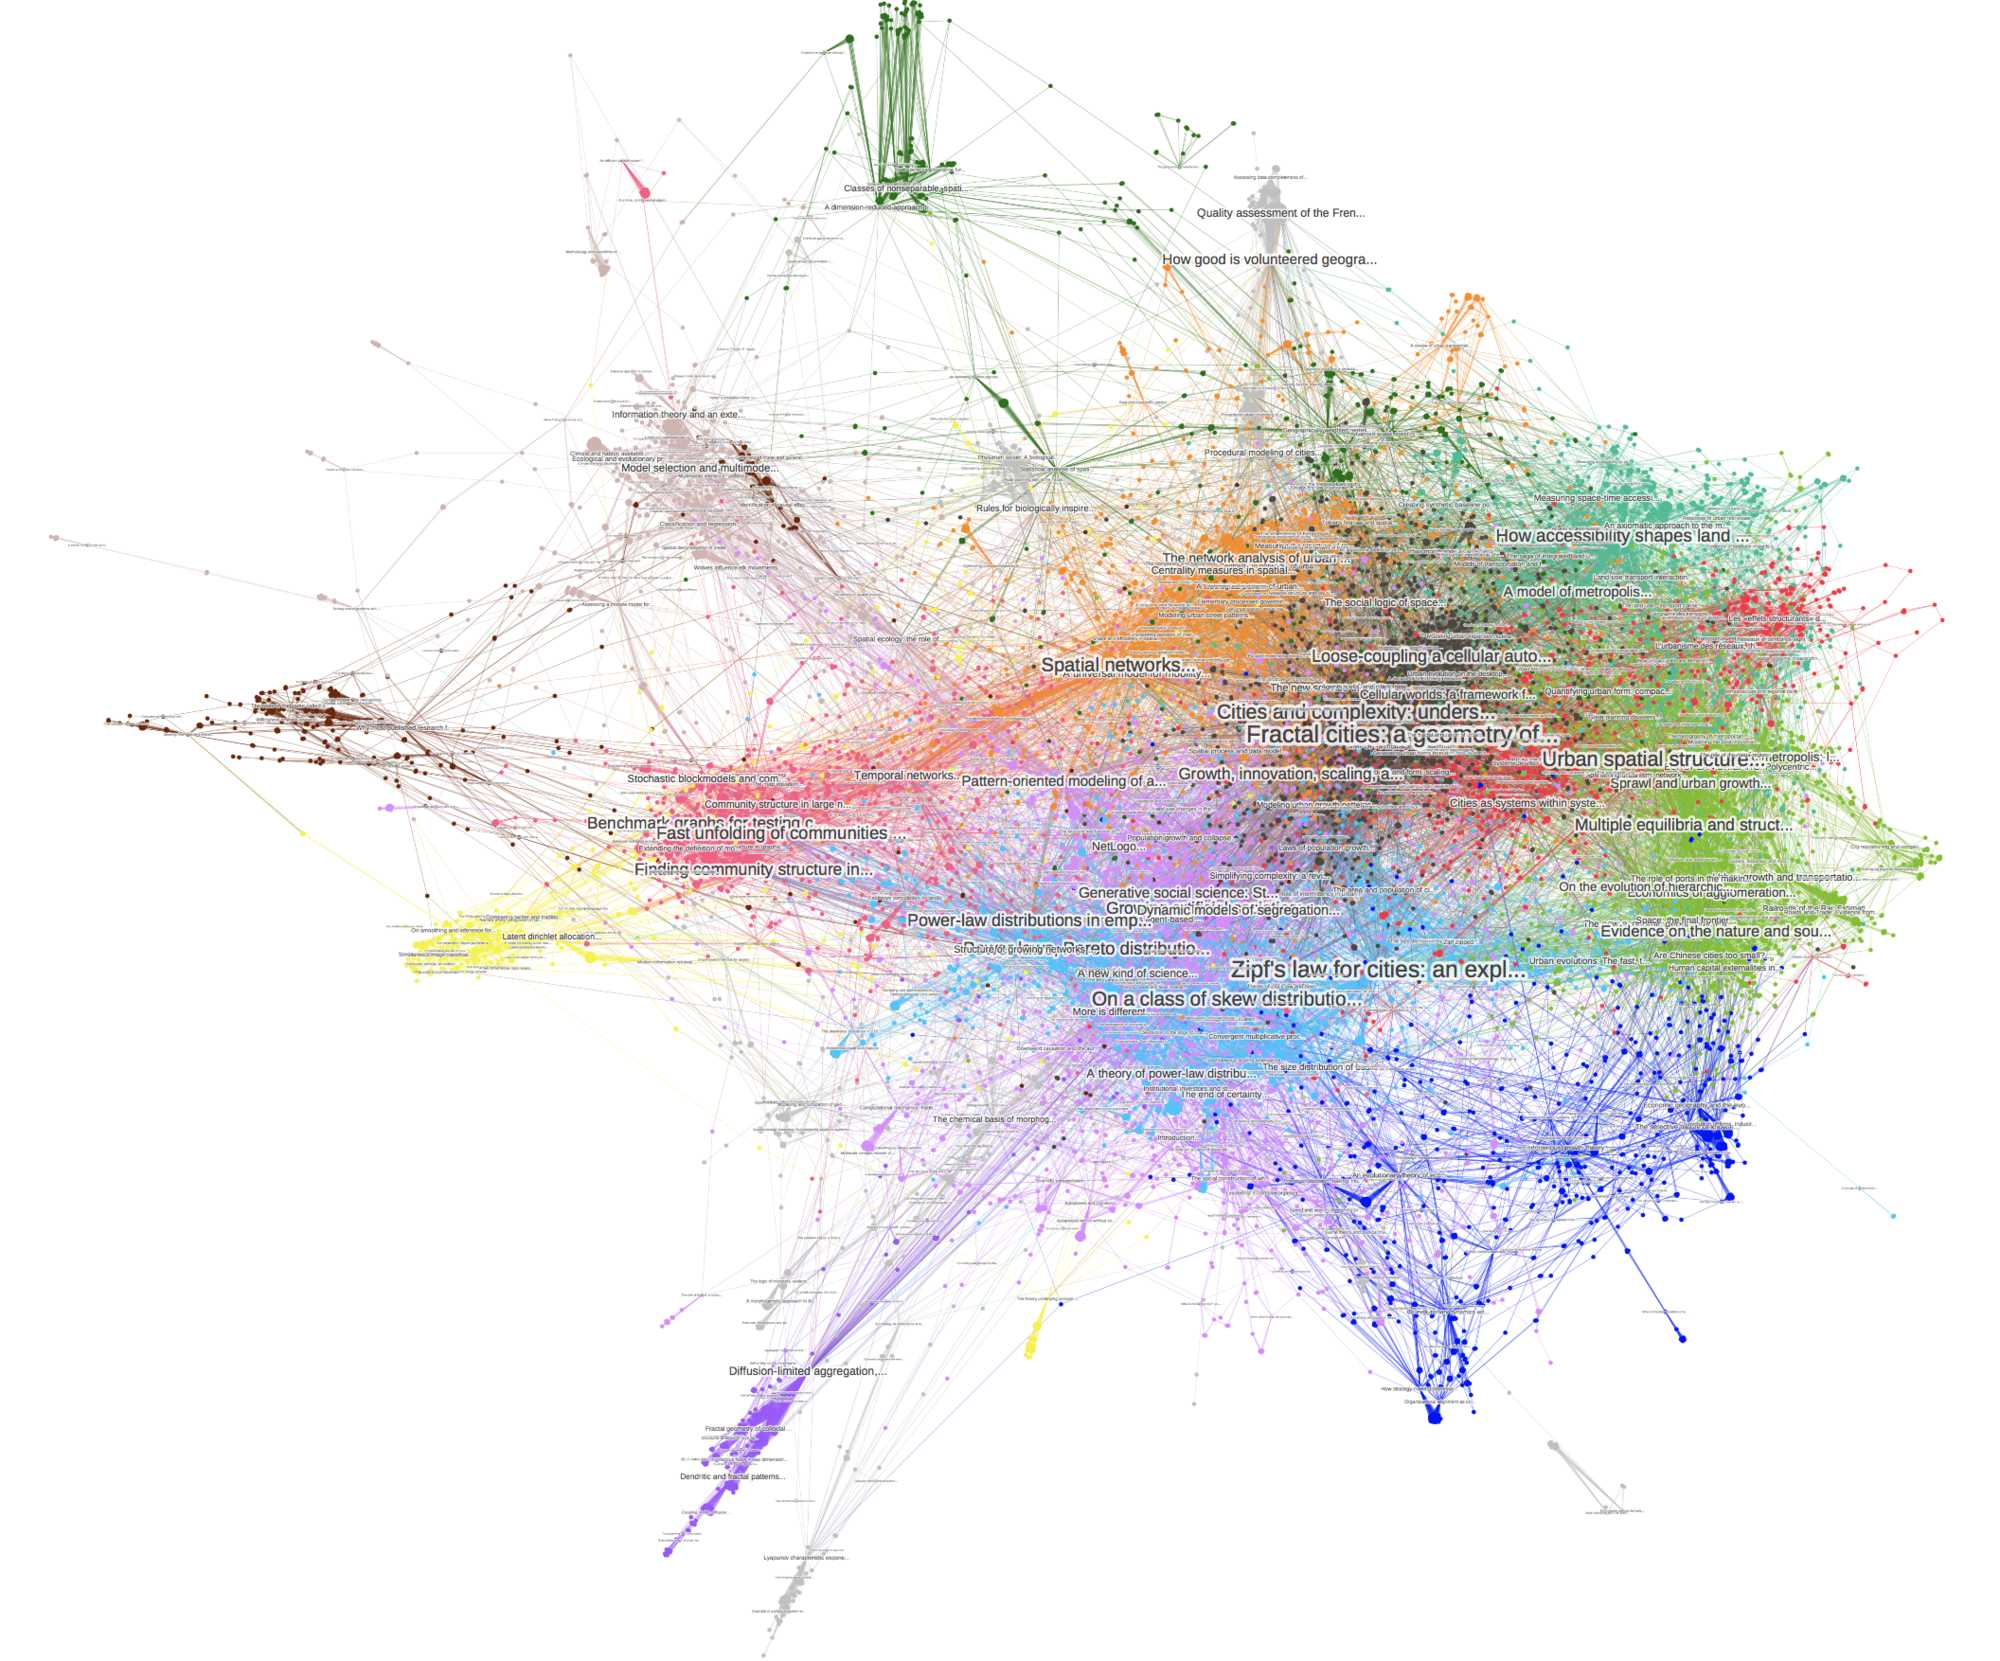
\includegraphics[width=\textwidth]{Figures/Final/F-reflexivity-citnw.jpg}
	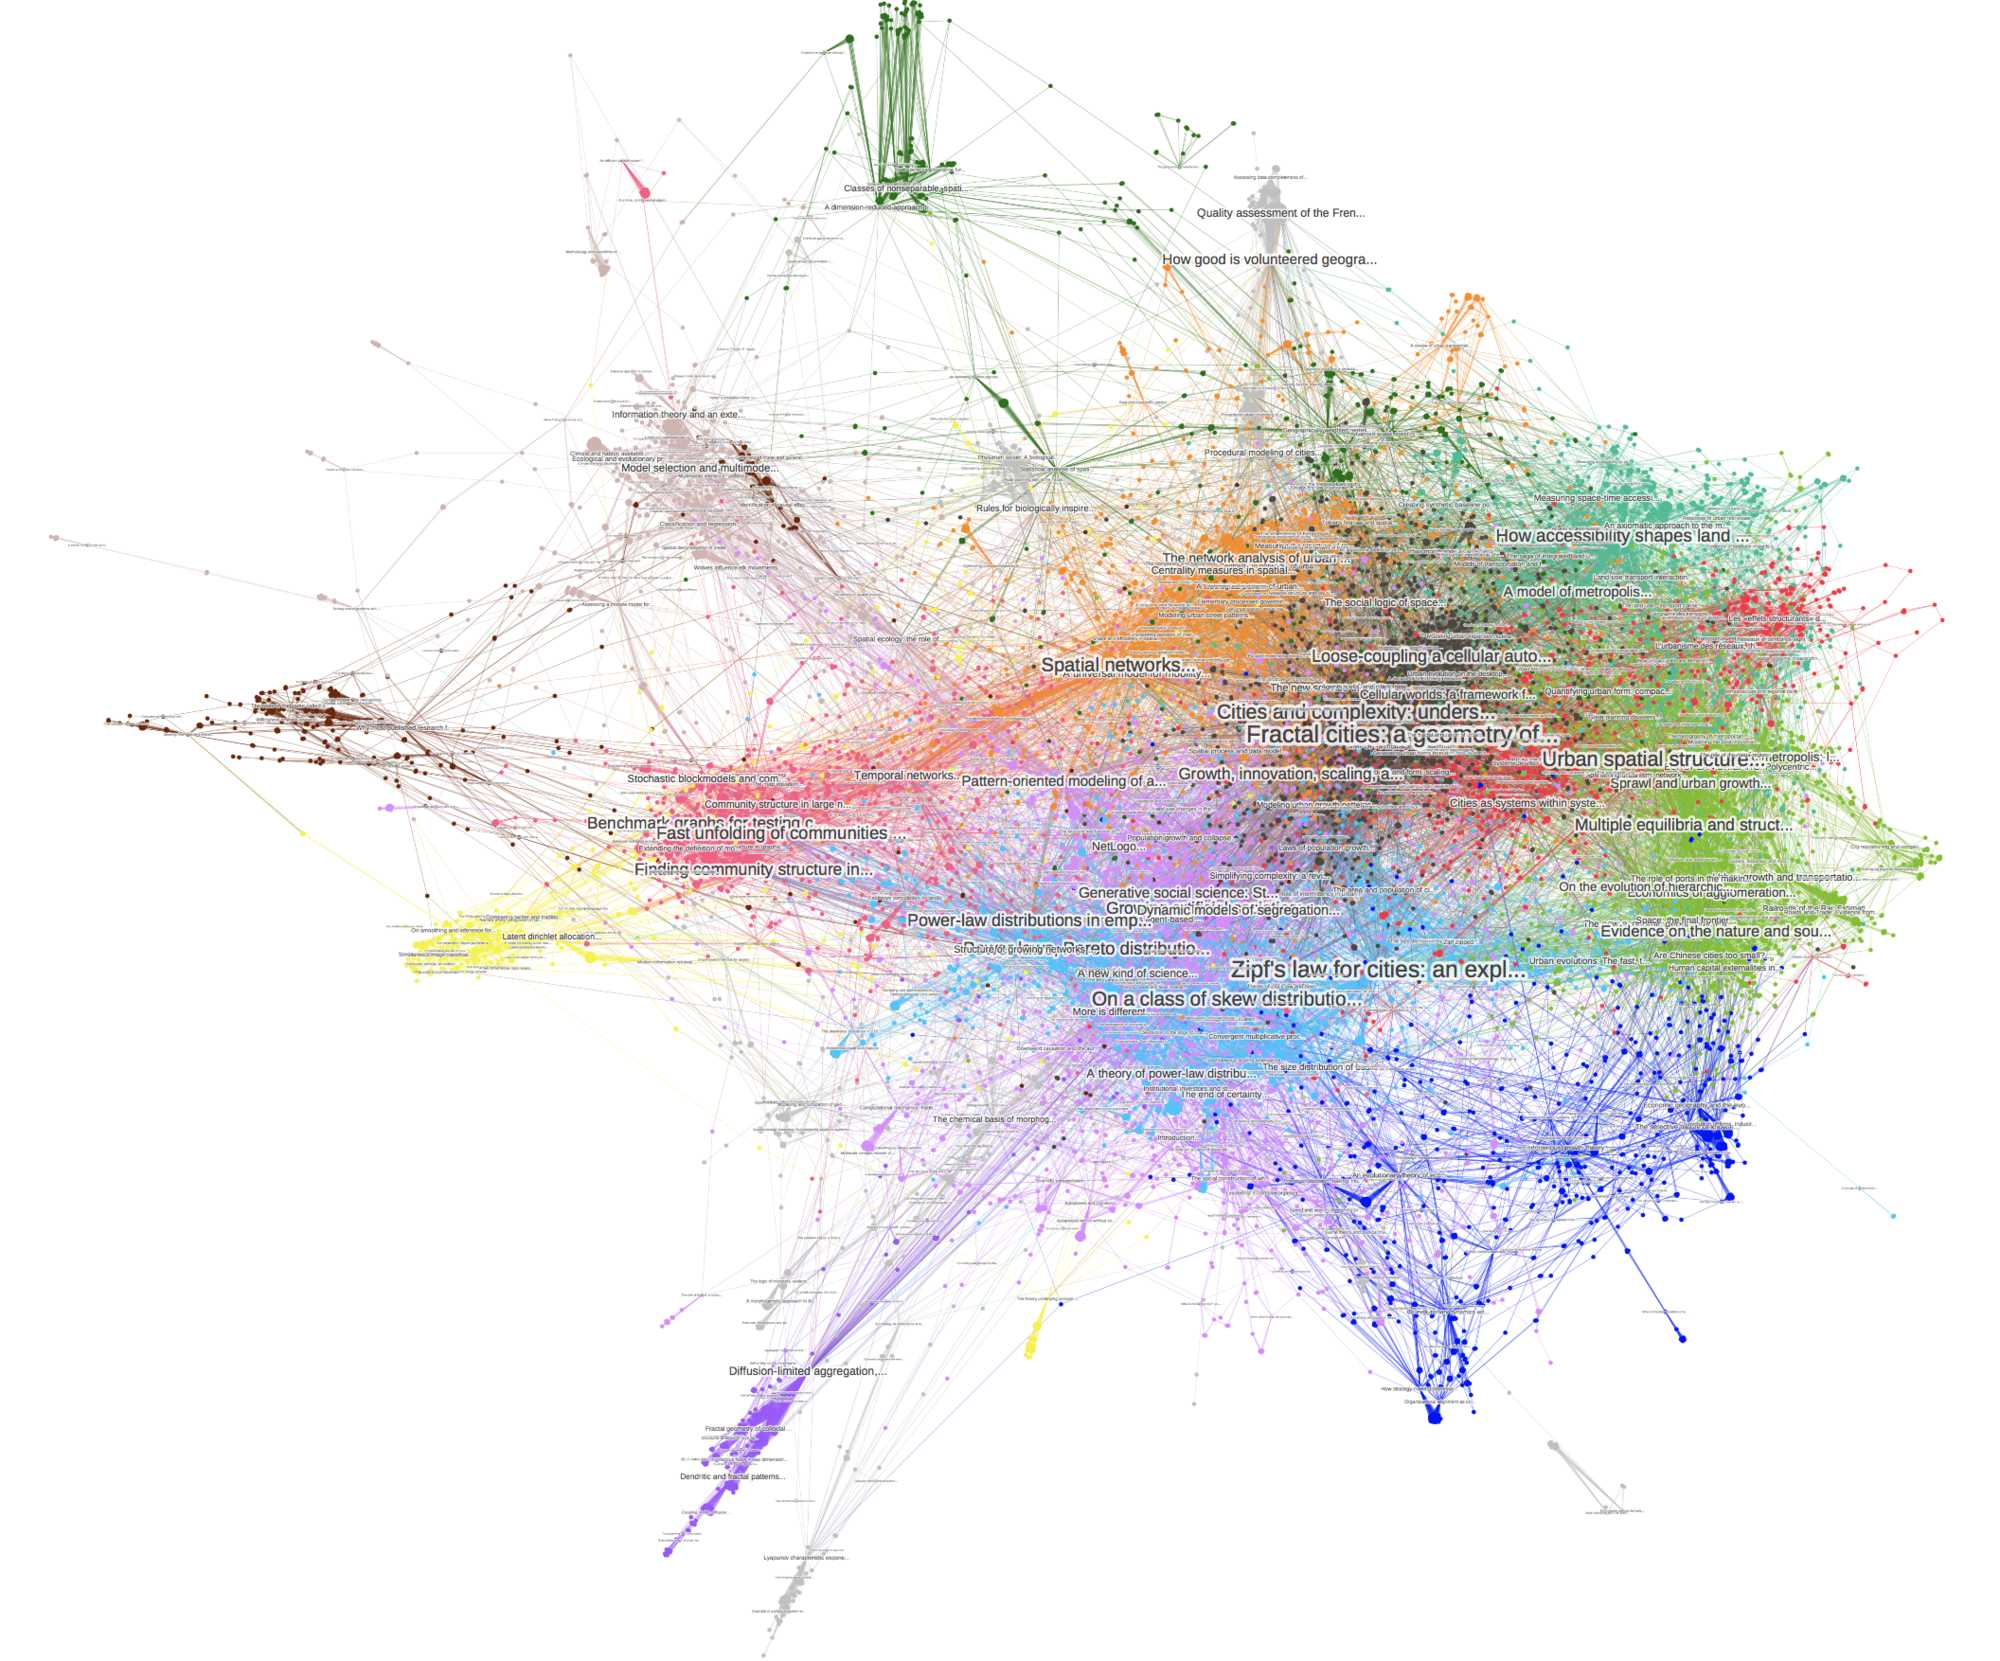
\includegraphics[width=\textwidth]{Figures/Final/F-reflexivity-citnw.jpg}
	\appcaption{\textbf{Citation network.}\label{fig:app:reflexivity:citnw}}{\textbf{Réseau de citation.}\label{fig:app:reflexivity:citnw}}
\end{figure}
%%%%%%%%%%%%



